\documentclass[border=10pt]{standalone}

\usepackage{tikz}
\usepackage{tikzsymbols}
\usetikzlibrary{calc,patterns,shapes.geometric}

\def\centerarc[#1](#2)(#3:#4:#5){\draw[#1] ($(#2)+({#5*cos(#3)},{#5*sin(#3)})$) arc (#3:#4:#5);}

\begin{document}
	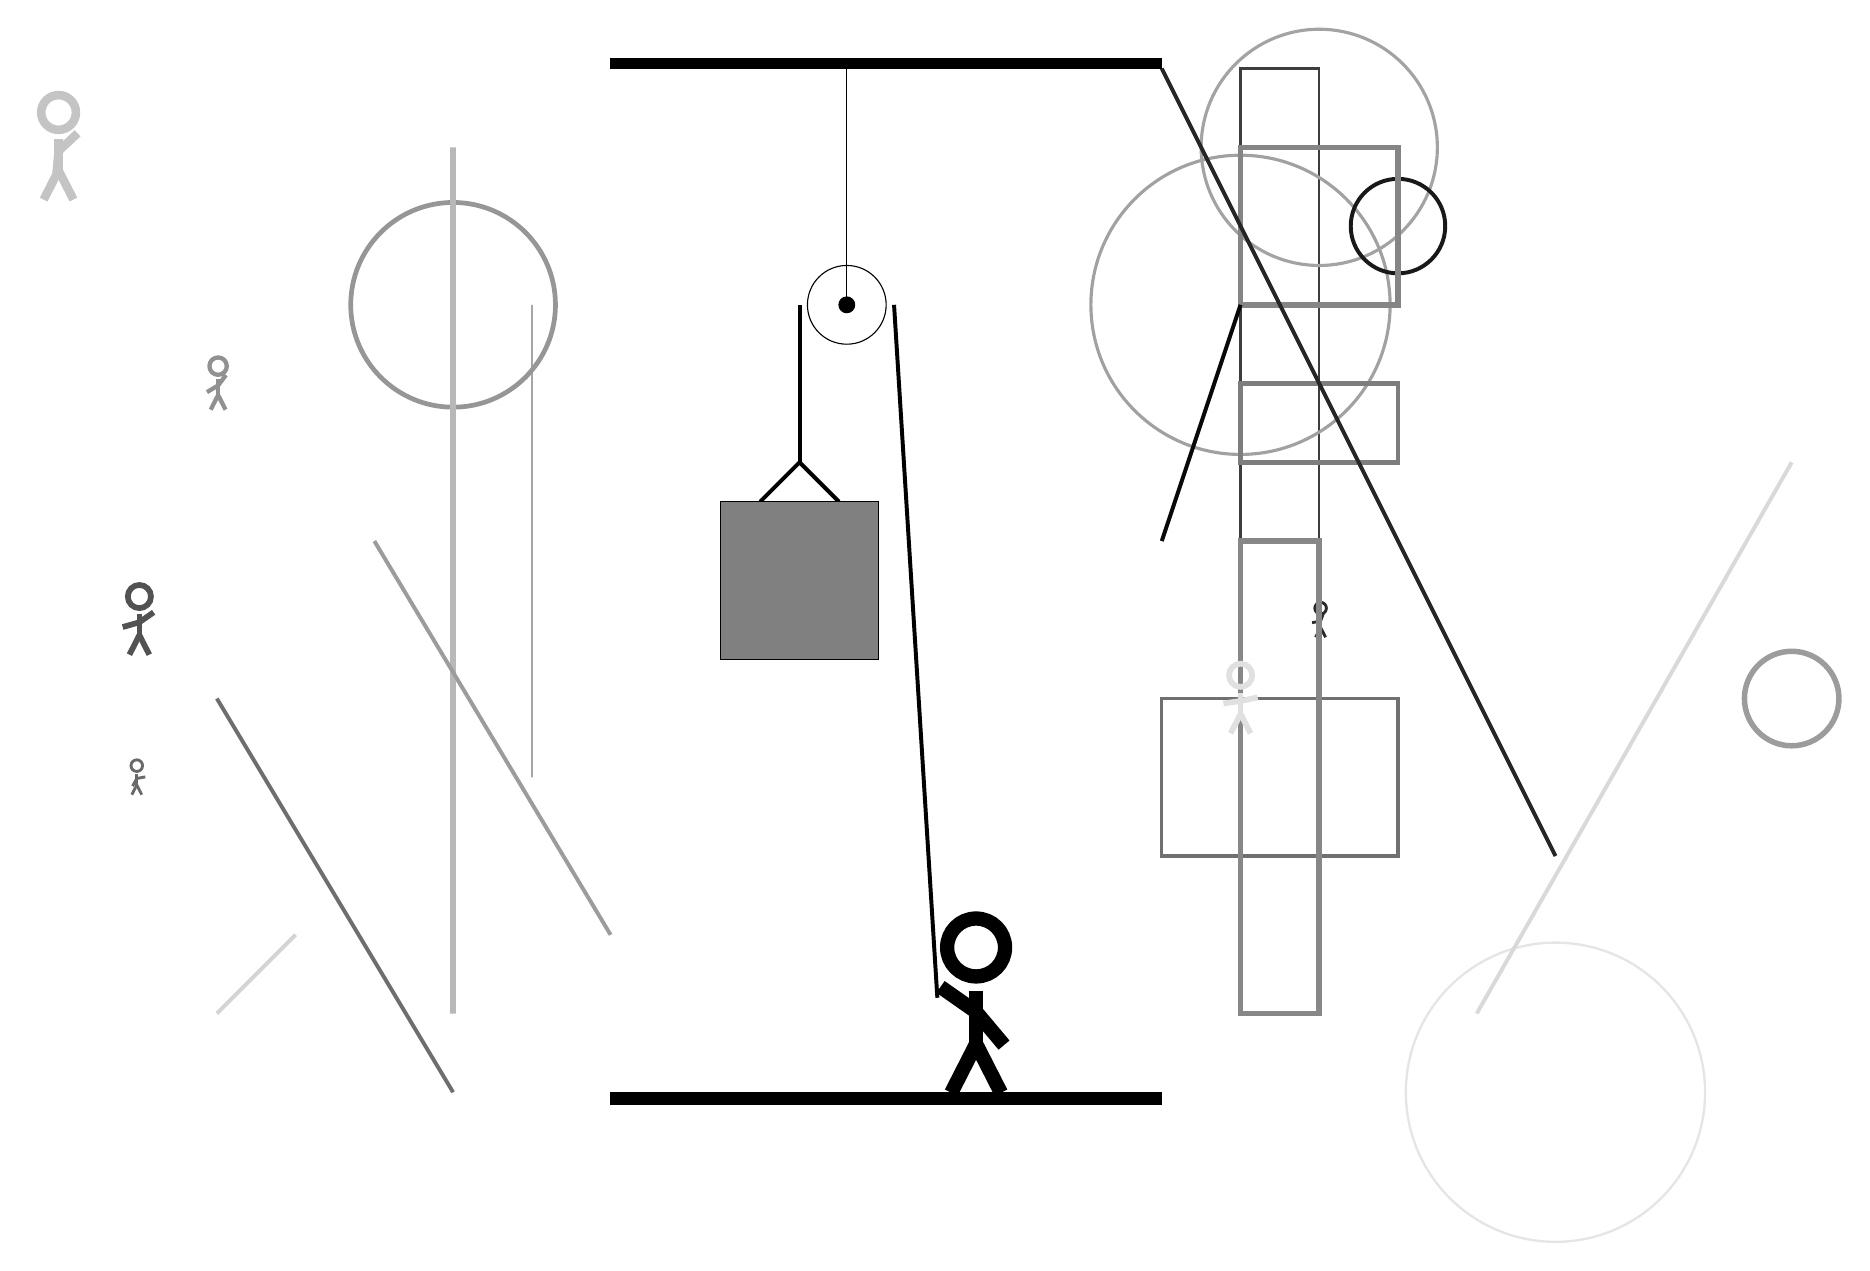
\begin{tikzpicture}
		%%%%% START %%%%%
		
		\draw[fill=black] (-2, 10) rectangle (5, 10.125);
		
		\draw (1, 7) circle (0.5);
		\draw[fill=black] (1, 7) circle (0.1);
		\draw (1, 10) -- (1, 7);
		
		\draw[line width=0.5mm] (-0.1, 4.5) -- (0.4, 5.0) -- (0.9, 4.5);
		\draw[fill=black!50] (-0.6, 4.5) rectangle (1.4, 2.5);
		
		\draw[line width=0.5mm] (0.4, 7) -- (0.4, 5.0);
		\centerarc[line width=0.5mm](1, 7)(0:180:0.6);
		\draw[line width=0.5mm](1.6, 7) -- (2.15, -1.8);
		
		\node at (2.6, -1.9) {\Strichmaxerl[10][-35][-50]};
		
		\draw[line width=0.4mm, color=black!56] (5, 2) rectangle (8, 0);
		
		\node[line width=0.5mm, color=black!83] at (7, 3) {\Strichmaxerl[2][11][70]};
		\draw[line width=0.3mm, color=black!76] (7, -2) rectangle (6, 10);
		\draw [line width=0.4mm, color=black!37](6, 7) circle (1.9);
		\node[line width=0.4mm, color=black!68] at (-8, 3) {\Strichmaxerl[4][16][35]};
		
		\draw[line width=0.7mm, color=black!47] (7, 4) rectangle (6, -2);
		\draw [line width=0.4mm, color=black!36](7, 9) circle (1.5);
		\draw [line width=0.3mm, color=black!10](10, -3) circle (1.9);
		\node[line width=0.4mm, color=black!59] at (-8, 1) {\Strichmaxerl[2][61][11]};
		\draw[line width=0.5mm, color=black!15](9, -2) -- (13, 5);
		\draw[line width=0.5mm, color=black!17](-7, -2) -- (-6, -1);
		\draw[line width=0.3mm, color=black!35] (-3, 1) rectangle (-3, 7);
		\node[line width=0.3mm, color=black!12] at (6, 2) {\Strichmaxerl[4][8][12]};
		
		\draw [line width=0.5mm, color=black!90](8, 8) circle (0.6);
		\draw [line width=0.7mm, color=black!39](13, 2) circle (0.6);
		\draw[line width=0.6mm, color=black!51] (6, 5) rectangle (8, 6);
		
		\node[line width=0.3mm, color=black!23] at (-9, 9) {\Strichmaxerl[6][85][43]};
		
		\draw[line width=0.7mm, color=black!48] (6, 7) rectangle (8, 9);
		\draw [line width=0.6mm, color=black!41](-4, 7) circle (1.3);
		\draw[line width=0.5mm, color=black!57](-4, -3) -- (-7, 2);
		\node[line width=0.6mm, color=black!43] at (-7, 6) {\Strichmaxerl[3][31][53]};
		
		\draw[line width=0.5mm, color=black!85](10, 0) -- (5, 10);
		
		\draw[line width=0.7mm, color=black!28] (-4, 9) rectangle (-4, -2);
		\draw[line width=0.5mm, color=black!97](6, 7) -- (5, 4);
		\draw[line width=0.5mm, color=black!39](-5, 4) -- (-2, -1);
		
		
		\draw[fill=black] (-2, -3) rectangle (5, -3.15);
		
		%%%%% END %%%%%
	\end{tikzpicture}
\end{document}